\documentclass[border=6pt]{standalone}
% Redrawn after Figure 4 of Verbitski et al., "Amazon Aurora: Design Considerations
% for High Throughput Cloud-Native Relational Databases", SIGMOD 2017.

% --- packages (mirror these in meta.json "requires") ---
\usepackage[T1]{fontenc}
\usepackage[scaled=0.92]{helvet}
\renewcommand{\familydefault}{\sfdefault}
\usepackage{tikz}
\usetikzlibrary{arrows.meta}

% --- colors sampled from the original figure ---
\definecolor{aunode}{HTML}{E2E2E2}
\definecolor{auinstance}{HTML}{B6DCFA}
\definecolor{auinstanceline}{HTML}{5C8DC5}
\definecolor{auinstancetext}{HTML}{3F7FBF}
\definecolor{aubackup}{HTML}{CAE9AB}
\definecolor{aubackupline}{HTML}{77B736}
\definecolor{aubackuptext}{HTML}{4F8A1F}
\definecolor{aucylinder}{HTML}{4A4A4A}
\definecolor{aucylindertop}{HTML}{949494}
\definecolor{aumark}{HTML}{4D4D4C}
\definecolor{auwire}{HTML}{6D6E6D}
\definecolor{autext}{HTML}{595959}
\definecolor{autitle}{HTML}{A6A6A6}
\definecolor{aurecorda}{HTML}{FCB64C}
\definecolor{aurecordb}{HTML}{007CBC}
\definecolor{aurecordc}{HTML}{B22491}
\definecolor{aupage}{HTML}{7BC233}

% ==== parameters (edit these) ============================================
\def\gridunit{0.0155}   % size of one layout unit (cm); scales the whole drawing
% labels
\def\titlelabel{STORAGE NODE}
\def\primarylabel{Primary\\Instance}
\def\peerlabel{Peer\\Storage\\Nodes}
\def\backuplabel{S3 BACKUP}
\def\incominglabel{INCOMING QUEUE}
\def\updatelabel{UPDATE\\QUEUE}
\def\hotloglabel{HOT\\LOG}
\def\datapageslabel{DATA\\PAGES}
\def\logrecordslabel{LOG RECORDS}
\def\acklabel{ACK}
\def\sortlabel{SORT\\GROUP}
\def\gossiplabel{PEER TO PEER GOSSIP}
\def\coalescelabel{COALESCE}
\def\gclabel{GC}
\def\scrublabel{SCRUB}
\def\snapshotlabel{POINT IN TIME\\SNAPSHOT}
% =========================================================================

\begin{document}
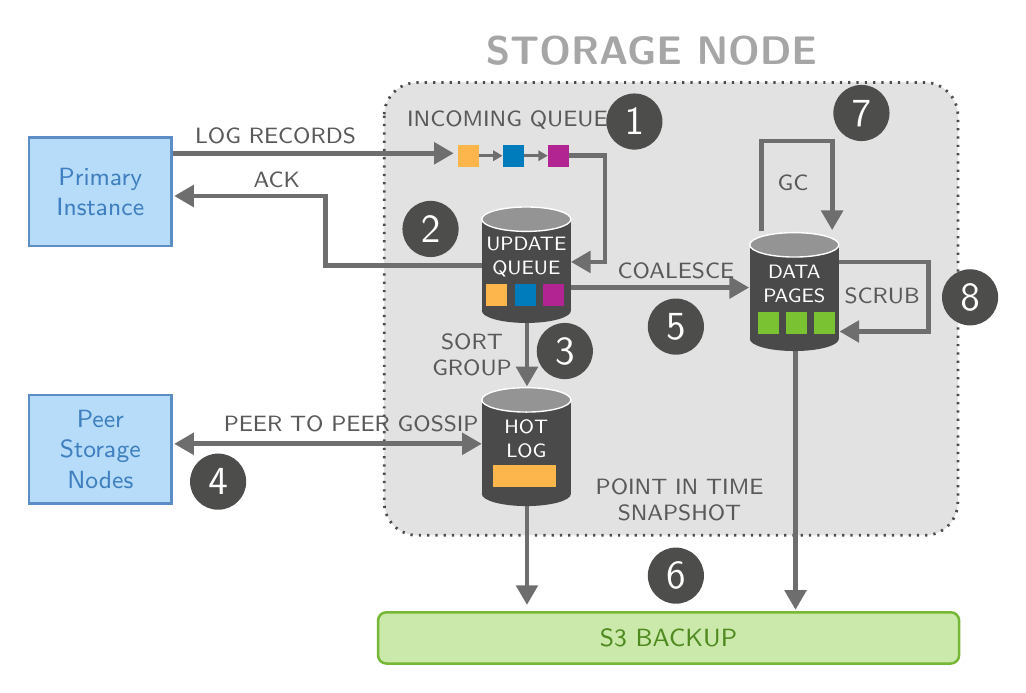
\begin{tikzpicture}[
    x=\gridunit cm, y=-\gridunit cm,
    >={Triangle[length=2.5mm, width=2.7mm]},
    font=\footnotesize,
    wire/.style={draw=auwire, line width=1.7pt},
    flow/.style={wire, ->},
    twoway/.style={wire, <->},
    thin flow/.style={draw=auwire, line width=1pt, -{Triangle[length=1.2mm, width=1.3mm]}},
    edge text/.style={text=autext, align=center, inner sep=0pt},
    instance/.style={
      draw=auinstanceline, line width=0.9pt, fill=auinstance, text=auinstancetext,
      font=\small, align=center, inner sep=0pt,
      minimum width=117*\gridunit cm, minimum height=89*\gridunit cm,
    },
    cyl text/.style={text=white, font=\fontsize{7.5}{8.5}\selectfont, align=center, inner sep=0pt},
    record/.style={inner sep=0pt, minimum width=17*\gridunit cm, minimum height=18*\gridunit cm},
    stepmark/.style={
      circle, fill=aumark, text=white, font=\Large, inner sep=0pt,
      minimum size=46*\gridunit cm,
    },
  ]

  % A store: node name, centre x, top y, bottom y.
  \newcommand{\store}[4]{
    \fill[aucylinder] (#2-36.5,#3+10) rectangle (#2+36.5,#4-10);
    \fill[aucylinder] (#2,#4-10) ellipse [x radius=36.5, y radius=10];
    \fill[aucylindertop, draw=white, line width=0.5pt] (#2,#3+10) ellipse [x radius=36.5, y radius=10];
    \node[inner sep=0pt, minimum width=73*\gridunit cm, minimum height={(#4-#3)*\gridunit cm}] (#1) at (#2,{(#3+#4)/2}) {};
  }

  % --- storage node and its neighbors ---
  \node[text=autitle, font=\Large\bfseries] (title) at (532,24) {\titlelabel};
  \draw[black!70, fill=aunode, line width=1pt, dash pattern=on 0.8pt off 2.2pt, rounded corners=12pt]
    (313,50) rectangle (783,421);
  \node[instance] (primary) at (80.5,139.5) {\primarylabel};
  \node[instance] (peer) at (80.5,350.5) {\peerlabel};
  \node[
    draw=aubackupline, line width=0.9pt, fill=aubackup, rounded corners=3pt, text=aubackuptext,
    font=\small, minimum width=476*\gridunit cm, minimum height=42*\gridunit cm, inner sep=0pt,
  ] (backup) at (546,505) {\backuplabel};

  % --- traffic ---
  \draw[flow] (140,108) -- (370,108);
  \node[edge text] at (224,94) {\logrecordslabel};
  \draw[flow] (394,200) -- (265,200) -- (265,143) -- (141,143);
  \node[edge text] at (225,130) {\acklabel};
  \draw[flow] (464,110) -- (494,110) -- (494,197) -- (466,197);
  \draw[flow] (430,247) -- (430,299);
  \node[edge text] at (385,273) {\sortlabel};
  \draw[flow] (465,218) -- (612,218);
  \node[edge text] at (552,204) {\coalescelabel};
  \draw[twoway] (141,346) -- (393,346);
  \node[edge text] at (286,330) {\gossiplabel};
  \draw[flow] (622,172) -- (622,98) -- (680,98) -- (680,171);
  \node[edge text] at (648,132) {\gclabel};
  \draw[flow] (685,197) -- (759,197) -- (759,254) -- (686,254);
  \node[edge text] at (721,225) {\scrublabel};
  \draw[flow] (430,397) -- (430,478);
  \draw[flow] (650,270) -- (650,482);
  \node[edge text] at (555,392) {\snapshotlabel};

  % --- incoming queue ---
  \node[edge text] at (414,81) {\incominglabel};
  \node[record, fill=aurecorda] (in1) at (382,110) {};
  \node[record, fill=aurecordb] (in2) at (419,110) {};
  \node[record, fill=aurecordc] (in3) at (456,110) {};
  \draw[thin flow] (in1) -- (in2);
  \draw[thin flow] (in2) -- (in3);

  % --- stores ---
  \store{update}{429.5}{152}{247}
  \node[cyl text] at (429.5,193) {\updatelabel};
  \node[record, fill=aurecorda] at (405,224) {};
  \node[record, fill=aurecordb] at (429,224) {};
  \node[record, fill=aurecordc] at (452,224) {};

  \store{hotlog}{429.5}{300}{397}
  \node[cyl text] at (429.5,342) {\hotloglabel};
  \foreach \x in {411,428,445} \node[record, fill=aurecorda] at (\x,372) {};

  \store{datapages}{649}{173}{270}
  \node[cyl text] at (649,215) {\datapageslabel};
  \foreach \x in {628,651,674} \node[record, fill=aupage] at (\x,247) {};

  % --- numbered steps ---
  \foreach \n/\x/\y in {1/518/82, 2/351/170, 3/461/270, 4/177/377, 5/552/250, 6/552/454, 7/704/75, 8/793/226}
    \node[stepmark] (step\n) at (\x,\y) {\n};

\end{tikzpicture}
\end{document}
